\documentclass[../../syllabus_2.tex]{subfiles}

\begin{document}
\chapter{Traitement de données}

\section{Activité d'introduction}

De combien d'enfants sont formées les familles des élèves de 2ème ?

\vspace{2cm}

Réorganisation des réponses :
%3 colonnes: variable, effectif et fréquance 

\begin{center}
    \begin{tblr}{
            hlines,
            vlines,
            columns={4cm, c},
            rows={1cm,m},
            row{1}={gray!40, font=\bfseries},
        }
         &  & \\
         &  & \\
         &  & \\
         &  & \\
         &  & \\
         &  & \\
         &  & \\
         &  & \\
         &  & \\
    \end{tblr}
\end{center}

Quelle est la moyenne pour la classe ?

\section*{Vocabulaire}

\begin{center}
    \begin{tblr}{
            hlines,
            vlines,
            colspec={lX[c]l},
            rows={2cm,m},
            row{1}={c, 1cm, gray!40, font=\bfseries},
            column{2}={7cm},
        }
        Mot                & Définition & Dans notre exemple \\
        Variable/caractère &            &                    \\
        Modalité           &            &                    \\
        Population         &            &                    \\
        Échantillon        &            &                    \\
        Effectif           &            &                    \\
        Effectif total     &            &                    \\
        Mode               &            &                    \\
        Étendue            &            &                    \\
    \end{tblr}
\end{center}

\newpage

\section{Applications}

\begin{exercise}
    L'association de Natura 2000 a proposé aux membres d'une association de prendre note des oiseaux qui passent dans leurs jardins au long d'une journée. Le tableau suivant reprend pour 6 oiseaux les observations de 5 participants.\\

    \begin{tblr}{hlines, vlines, hline{1}={1}{white}, vline{1}={1}{white},colspec={l*{6}{X[c]}}, row{1}={m}}
               & Merle noir & Mésange & Rouge-gorge & Moineau & Pie & Tourterelle \\
        Bruno  & 3          & 4       & 1           & 6       & 2   & 0           \\
        Luc    & 3          & 6       & 3           & 4       & 3   & 1           \\
        Myriam & 5          & 2       & 6           & 5       & 3   & 3           \\
        Clara  & 4          & 3       & 2           & 4       & 2   & 4           \\
        Matis  & 6          & 5       & 3           & 7       & 4   & 2           \\
    \end{tblr}\\

    \begin{enumerate}
        \item Complète le tableau suivant.
              \begin{center}
                  \begin{tblr}{hlines, vlines, hline{1}={1}{white}, vline{1}={1}{white},width=.75\linewidth,colspec={lX[c]X[c]}}
                                  & Effectif & Fréquence(en pourcentages, à l'unité près) \\
                      Merle noir  & 21       &                                            \\
                      Mésange     &          &                                            \\
                      Rouge-gorge &          &                                            \\
                      Moineau     &          &                                            \\
                      Pie         &          &                                            \\
                      Tourterelle &          &                                            \\
                      Totaux      &          &                                            \\
                  \end{tblr}
              \end{center}
        \item Quel est le mode ?\\
              \vspace{1cm}
        \item Quel est le type de variable ?\\
              \vspace{1cm}
              % On introduit quelque part les types de variables ?
        \item Quelle est, en moyenne, le nombre d'oiseaux vus par une personne ?
    \end{enumerate}
    \vspace*{2cm}
\end{exercise}

\newpage
\begin{exercise}
    On étudie les résultats de l'examen de math des élèves de 2ème de l'école Status. \\
    Voici les cotes obtenues par les élèves de la classe de 2ème G.

    \tcbsidebyside[blanker, sidebyside align=top seam, sidebyside adapt=left]{%
        \begin{tblr}{
                hlines,
                vlines,
                rows={m},
            }
            Albus   & 8  \\
            Bloem   & 2  \\
            Ducobu  & 0  \\
            Dupont  & 4  \\
            Enigma  & 6  \\
            Fabulus & 7  \\
            Granger & 8  \\
            Gratin  & 10 \\
            Joker   & 9  \\
            Lux     & 7  \\
            Potter  & 8  \\
            Romain  & 6  \\
            Twix    & 6  \\
            Wisley  & 8  \\
            Zak     & 2  \\
        \end{tblr}
    }{%
        \begin{enumerate}[itemsep=2.5cm]
            \item Quelle est la population observée ?
            \item Quel est l'échantillon observé ?
            \item Quel est le caractère observé ?
            \item Ce caractère est-il quantitatif ou qualitatif ?
            \item Quelle est l'étendue de cette série ?
            \item Quel est l'effectif total ?
                  \setcounter{mycounterlist}{\value{enumi}}
        \end{enumerate}
        \vspace*{2,5cm}
    }
    \newpage
    \begin{enumerate}
        \setcounter{enumi}{\value{mycounterlist}}
        \item Complète le tableau de distribution des cotes des élèves de 2G ci-dessous. \\
              \begin{center}
                  \begin{tblr}{
                          hlines,
                          vlines,
                          colspec={*{3}{X[c]}},
                          rows={0.8cm,m},
                          row{1}={gray!40, font=\bfseries},
                      }
                      Modalités & Effectifs & Fréquences (en \%) \\
                               &          &                   \\
                               &          &                   \\
                               &          &                   \\
                               &          &                   \\
                               &          &                   \\
                               &          &                   \\
                               &          &                   \\
                               &          &                   \\
                               &          &                   \\
                               &          &                   \\
                               &          &                   \\
                               &          &                   \\
                  \end{tblr}
              \end{center}

        \item Trace le diagramme en bâtonnets qui représente la répartition des notes pour les élèves de 2G. \\
              
\includegraphics[width=\linewidth]{img/quadrillage.png}
    \end{enumerate}
\end{exercise}

\newpage
\begin{exercise}
    Quelle couleur les Bruxellois choisissent-ils pour leur voiture ? On a interrogé le garage « Thomas et fils » et voici un graphique de ses ventes en 2021. \\
    \begin{center}
        
\includegraphics{img/voitures.png}
    \end{center}

    \begin{enumerate} [itemsep=1.5cm]
        \item Quelle est la population observée ?
        \item Quel est l'échantillon observé ?
        \item Quel est le caractère observé ?
        \item Ce caractère est-il quantitatif ou qualitatif ?
        \item Quel est l'effectif total ?
        \item Quelle est la probabilité    \footnote{La probalité represente la possibilité qu'un évenement se produise.} qu'une voiture vendue prise au hasard soit bleue ?
              \newpage
        \item Peut-on calculer l'étendue de cette série ?
        \item Complète le tableau de distribution des couleurs de voitures du garage de « Thomas et fils » et calcule l'amplitude des angles afin de tracer un diagramme circulaire. \\

              \begin{tblr}{hlines, vlines, colspec={*{4}{X[c]}}, rows={m, 1cm}}
                  Modalités & Effectifs & Fréquences & Amplitudes \\
                           &          &           &           \\
                           &          &           &           \\
                           &          &           &           \\
                           &          &           &           \\
                           &          &           &           \\
                           &          &           &           \\
              \end{tblr}
        \item Trace le diagramme circulaire de la situation dans un cercle de $3 cm $ de rayon. N'oublie pas ta légende !

    \end{enumerate}

\end{exercise}

\newpage
\begin{exercise}
    Voici un tableau de distribution. Les affirmations sont-elles vraies ou fausses? Justifie.
    \begin{center}
        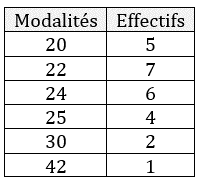
\includegraphics{img/tableua.png}
    \end{center}
    \begin{enumerate}[cols=2, itemsep = 2cm]
        \item L'effectif total est 163.
        \item 30\% est la fréquence \\de la modalité 22.
        \item Le mode est 42.
        \item La moyenne est 24.
        \item L'étendue est 22.
    \end{enumerate}
\end{exercise}

\vspace*{1cm}

\begin{exercise}
    Voici les températures maximales en degrés Celsius relevées à Bizeneuille au cours du mois de juillet de l'été dernier. \\
    Détermine le mode et calcule la moyenne au dixième près de cette série statistique.

    \begin{tblr}{hlines, vlines, colspec={l*{9}{X[c]}}}
        Température     & 32 & 33 & 34 & 35 & 36 & 37 & 38 & 39 & 40 \\
        Nombre de jours & 1  & 1  & 4  & 7  & 2  & 5  & 6  & 2  & 3  \\
    \end{tblr}
\end{exercise}

\newpage
\begin{exercise}
    Trente personnes du même club ont recensé le nombre d'oiseaux observés dans leur jardin durée dans la même journée. Leurs observations sont présentées sous la forme d'un diagramme en bâtons qu'elles ont communiqué à Natura 2000.
    \begin{center}
        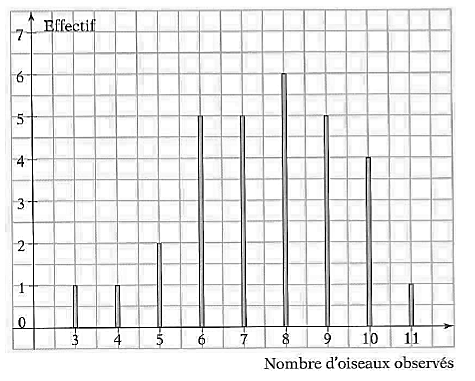
\includegraphics[]{img/natura.png}
    \end{center}

    \begin{enumerate} [cols=2, itemsep = 2cm]
        \item Combien de personnes ont observé cinq oiseaux?
        \item Quel est le mode?
        \item Quel est le nombre minimum d'oiseaux observés ?
        \item En tout, combien d'oiseaux a-t-on observé durant cette journée?
        \item Quel est, en moyenne, le nombre d'oiseaux observés par une personne ?
        \item Combien de personnes ont observé un nombre d'oiseaux supérieur à la moyenne?
    \end{enumerate}
\end{exercise}

\newpage
\begin{exercise}
    Dans une classe de 25 élèves, on a noté la somme d'argent de poche que reçoit chaque élève par semaine. Complète le tableau et réponds aux questions.  \\
    \begin{tblr}{hlines, vlines, colspec={l*{6}{X[c]}}}
        Somme en €      & 2 & 5 & 8  & 11 & 14 & 17 \\
        Nombre d'élèves & 2 & 7 &    &    &    &    \\
        Fréquence en \% &   &   & 24 & 20 & 16 & 4  \\
    \end{tblr}

    \begin{enumerate} [ itemsep = 0.7cm]
        \item Quel est l'effectif total?
        \item Quel est le type de variable?
        \item Quelle est l'étendue?
        \item Quel est l'effectif pour la somme de $11$ euros ?
        \item Quelle est la moyenne d'argent de poche qu'un élève de cette classe reçoit?
    \end{enumerate}

\end{exercise}

\vspace*{2cm}

\begin{exercise}
    Camille a obtenu trois cotes sur 20 (12, 17 et 16) en mathématiques pour le bulletin de la dernière période. Son professeur a donné autant d'importance à chaque interrogation. Mais en fin de période, le professeur a décidé d'organiser un bilan dont l'importance est double par rapport à chaque interrogation précédente. \\ Combien Camille doit-elle obtenir à cette interrogation pour avoir une moyenne de 80\% ?
\end{exercise}

\newpage

\begin{exercise}
    Tous les élèves de 2ème année d'une école ont assisté à une pièce de théâtre. A la fin du spectacle, on leur a demandé d'attribuer une cote sur 20 traduisant la qualité de la représentation. Voici le tableau des résultats.

    \begin{tblr}{hlines, vlines, colspec={l*{9}{X[c]}}}
        Cotes            & 4 & 8  & 9  & 12 & 13 & 15 & 16 & 17 & 19 \\
        Nombres d'élèves & 3 & 15 & 23 & 13 & 21 & 21 & 35 & 14 & 7  \\
    \end{tblr}

    \begin{enumerate}[itemsep=5cm]
        \item Détermine le mode et calcule la moyenne de cette série statistique.
        \item Les professeurs de l'école estiment qu'un spectacle scolaire est une réussite si la moitié des élèves ont attribué une cote d'au moins 14/20. Tenant compte de cette affirmation, peux-tu dire si ce spectacle a été une réussite ? Explique.
        \item Quant aux acteurs de la troupe, ils estiment avoir bien joué leur rôle si seulement un quart des élèves au maximum ont attribué une cote en dessous de 10. Les acteurs peuvent-ils être satisfaits de leur prestation ? Explique.

    \end{enumerate}
\end{exercise}

\newpage
\begin{exercise}
    Un agent immobilier prévoit de promouvoir la ville de \textit{Lounialand}. Pour ça, il a besoin de faire quelques relevés. \\ Voici les surfaces habitables, en $m^2$, des neuf maisons du quartier de \textit{La Calista}.

    \begin{tblr}{hlines, vlines, colspec={*{9}{X[c]}}}
        82 & 104 & 107 & 126 & 196 & 210 & 225 & 230 & 250
    \end{tblr}

    \begin{enumerate}[cols = 2, itemsep = 2cm]
        \item Quel est l'effectif total?
        \item Quelle est la population?
        \item Quel est l'échantillon?
        \item Quel est le caractère?
        \item Quel est le type de caractère?
        \item Quelle est, en moyenne, la surface habitable d'une maison de ce quartier?
    \end{enumerate}
    \vspace{3cm}
\end{exercise}

\begin{exercise}
    Ce graphique donne des renseignements à propos de la randonnée à vélo que Tobias a faite dimanche dernier. \\

    \begin{enumerate}[cols = 2, itemsep = 1cm]
        \item [\label=]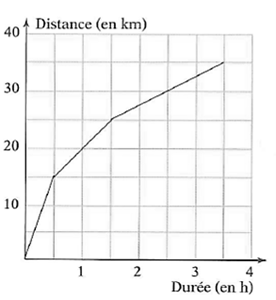
\includegraphics[]{img/velo.png}
        \item Quelle est la distance parcourue?
        \item Quelle est la durée de son trajet?
        \item A quelle vitesse Tobias a-t-il parcouru le dernier tronçon?
        \item Quelle est sa vitesse moyenne sur l'ensemble du parcours?
    \end{enumerate}
\end{exercise}

\newpage
\begin{exercise}
    La liste ci-dessous reprend les tailles de chaussures d'une équipe de football (avec les réservistes).
    \begin{center}
        42  -  44  -  43  -  44  -  45  -  47  -  46  -  40  -  44  -  45  -  44  -  46  -  45
    \end{center}
    \begin{enumerate}[itemsep=1cm]
        \item Remplis le tableau ci-dessous. \\
              \begin{tblr}{hlines, vlines, colspec={*{3}{X[c]}}, rows={0.8cm}}
                  Taille des chaussures & Nombre de joueurs & Fréquences \\
                                        &                   &            \\
                                        &                   &            \\
                                        &                   &            \\
                                        &                   &            \\
                                        &                   &            \\
                                        &                   &            \\
                                        &                   &            \\
                                        &                   &            \\
                                        &                   &            \\
              \end{tblr}
        \item Dans quelle colonne observe-t-on les effectifs?
        \item Quel est le type de variable?
        \item Quel est l'effectif total?
        \item Quel est le mode?
        \item Quelle est l'étendue?
        \item Quelle est la moyenne des pointures? Écris ton calcul.
    \end{enumerate}

\end{exercise}

\newpage
\section{Exercices issus de CE1D}

\begin{exercise}
    Trois seaux contiennent chacun 40 billes de trois couleurs différentes : rouges, vertes et bleues. Elles sont indiscernables au toucher. Dans chaque seau, la répartition des billes est différente. Pour chacune des expériences ci-dessous, on tire une bille au hasard.
    \begin{enumerate}[itemsep=4cm]
        \item Dans le premier seau, la probabilité de tirer une bille rouge est de 25 \%. \\Détermine le nombre de billes rouges contenues dans le seau.
        \item Dans le deuxième seau, la probabilité de tirer une bille rouge est de 0,6 et celle de tirer une verte est de 20\%. \\Détermine le nombre de billes bleues contenues dans le seau.
        \item Dans le dernier seau, la probabilité de tirer une bille bleue est de 5\% et il y a autant de billes vertes que de billes rouges. \\Détermine le nombre de billes vertes contenues dans ce seau.
              \vspace*{3cm}
    \end{enumerate}
\end{exercise}

\newpage

\begin{exercise}
    La bibliothécaire de l'école a fait un relevé du nombre de livres empruntés par les élèves pendant un trimestre. Voici les résultats.\\

    \begin{tblr}{hlines, vlines, colspec={l*{5}{X[c]}}}
        Nombre de livres empruntés & 1    & 2    & 3    & 4    & 5    \\
        Fréquence                  & 14\% & 22\% & 18\% & 34\% & 12\% \\
    \end{tblr}

    \begin{enumerate}[itemsep=4cm]
        \item Sachant que 216 élèves ont emprunté trois livres à la bibliothèque, quel est le nombre total d'élèves ayant emprunté au moins un livre au cours de ce trimestre ?
        \item Quel est le nombre moyen de livres empruntés par un élève s'étant rendu à la bibliothèque au cours de ce trimestre ?
              \vspace*{3cm}
    \end{enumerate}
\end{exercise}



\begin{exercise}
    Sur cette grille de combat naval, Nelson a placé quatre bateaux. Lors du 1er tir, son adversaire désigne au hasard l'une des cases de la grille. \\
    Quelle est la probabilité :

    \begin{enumerate} [cols=2, itemsep = 2cm]
        \item Qu'un bateau soit touché ?
        \item Qu'une case voisine (par un côté ou un sommet) d'un bateau soit touchée ?
        \item Que ni un bateau, ni une case voisine ne soit atteinte ?
        \item [\label=] 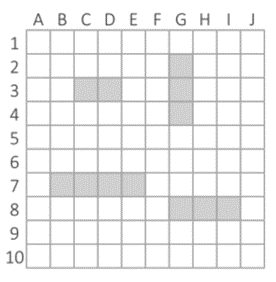
\includegraphics[]{img/combat_naval.png}
              \vspace*{2cm}
    \end{enumerate}
\end{exercise}

\newpage
\begin{exercise}
    \par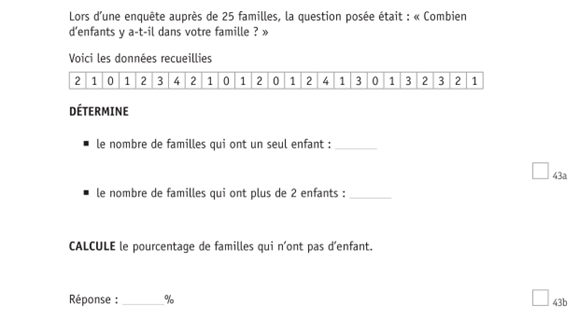
\includegraphics[]{img/CE1D7.png}
\end{exercise}

\newpage
\begin{exercise} 
    \par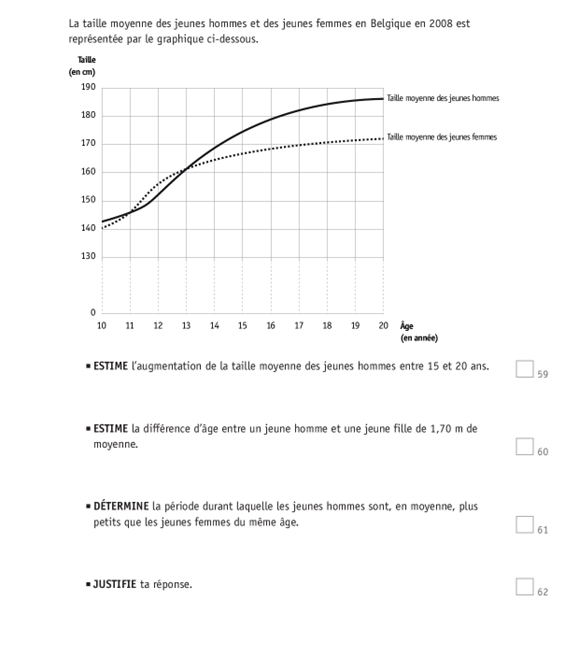
\includegraphics[]{img/CE1D1.png}
\end{exercise}

\newpage
\begin{exercise} 
    \par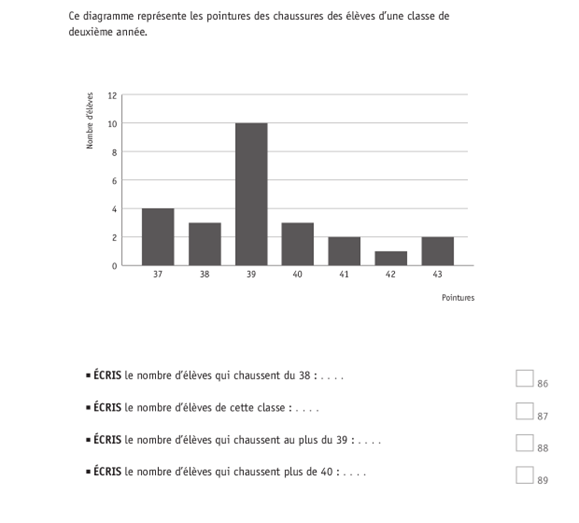
\includegraphics[]{img/CE1D2.png}
\end{exercise}

\newpage
\begin{exercise}
    \par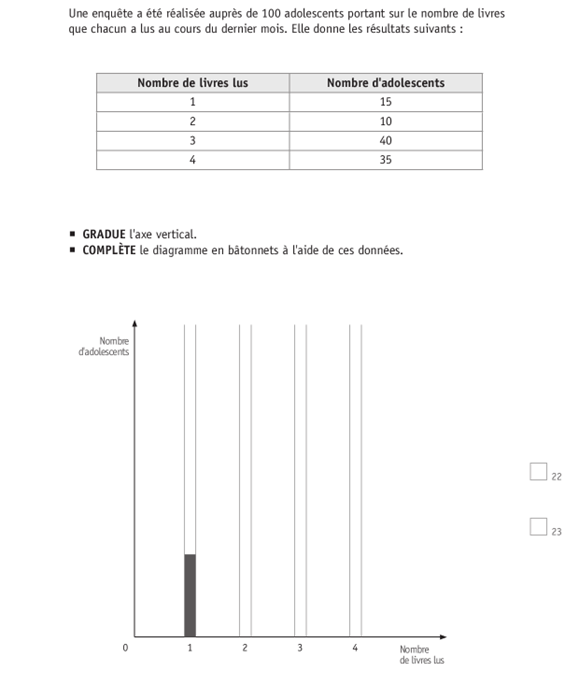
\includegraphics[]{img/CE1D3.png}
\end{exercise}

\newpage
\begin{exercise}
    \par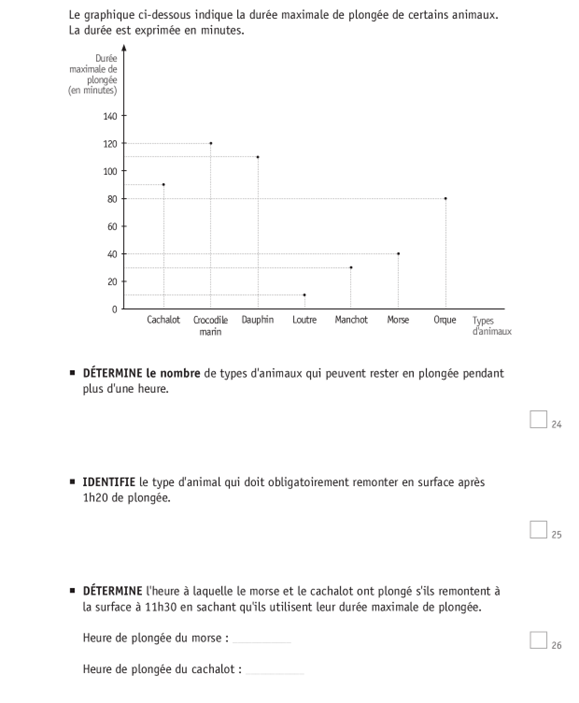
\includegraphics[]{img/CE1D4.png}
\end{exercise}

\newpage
\begin{exercise}
    \par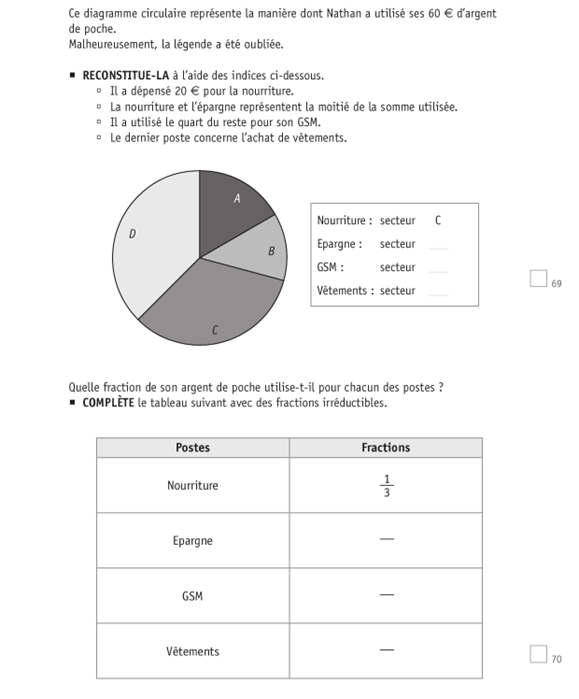
\includegraphics[]{img/CE1D5.png}
\end{exercise}

\newpage
\begin{exercise}
    \par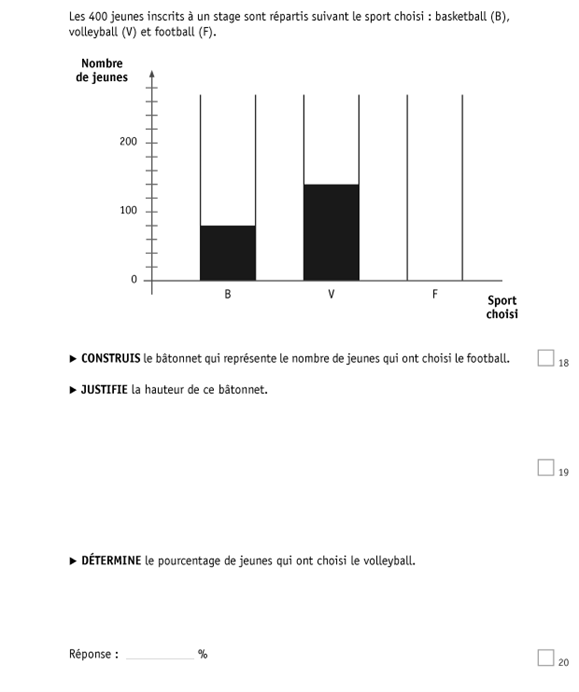
\includegraphics[]{img/CE1D6.png}
\end{exercise}

\newpage
\begin{exercise}
    \par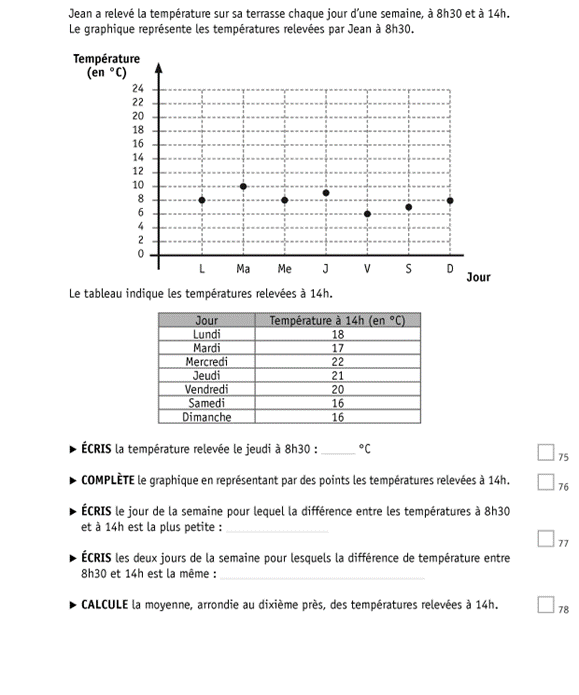
\includegraphics[]{img/CE1D8.png}
\end{exercise}

\newpage
\begin{exercise}
    \par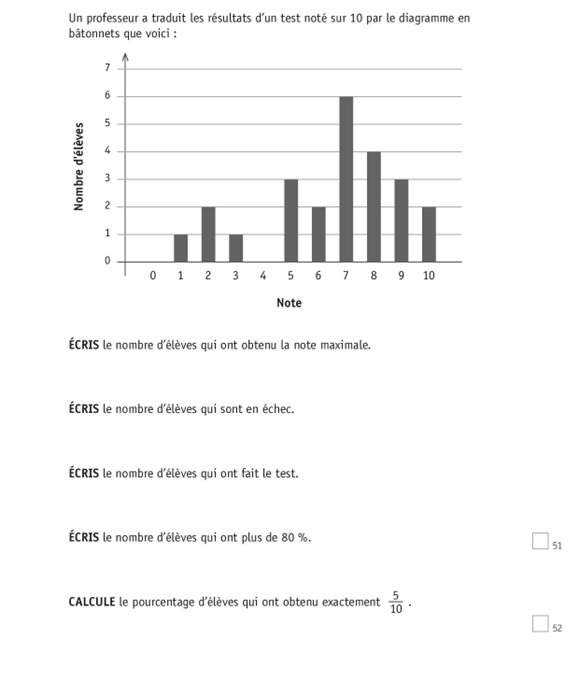
\includegraphics[]{img/CE1D9.png}
\end{exercise}

\newpage
\begin{exercise}
    \par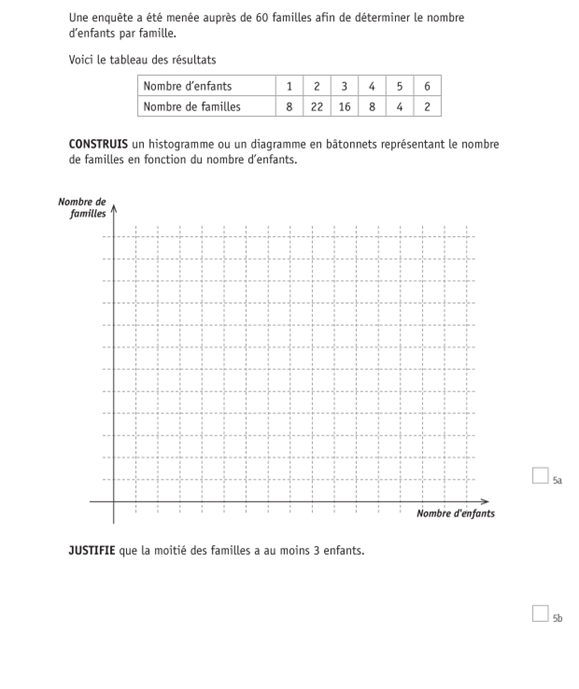
\includegraphics[]{img/CE1D10.png}
\end{exercise}

\newpage
\begin{exercise}
    \par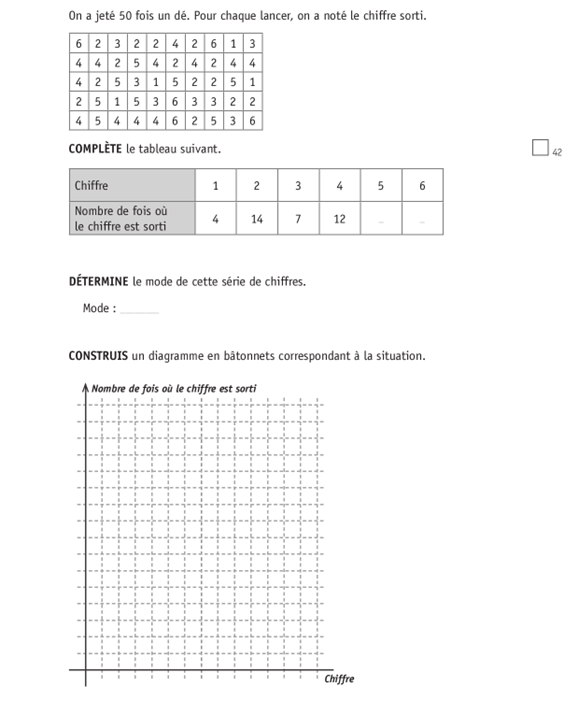
\includegraphics[]{img/CE1D11.png}
\end{exercise}
\end{document}